\documentclass[12pt,a4paper]{article}
\pdfoutput=1

\usepackage[utf8]{inputenc}
\usepackage[T1]{fontenc}
\usepackage[swedish]{babel}
\usepackage{amsmath}
\usepackage{lmodern}
\usepackage{units}
\usepackage{icomma}
\usepackage{color}
\usepackage{graphicx}
\usepackage{multicol,caption}
\usepackage{bbm}
\usepackage{hyperref}
\usepackage{xfrac}
\usepackage{listings}
\usepackage{multirow}
\usepackage{fancyhdr}
\pagestyle{fancy}
\lhead{Stereoskopisk snösimulering}
\rhead{\today}

\begin{document}

\begin{center}

	{ \huge \bfseries Stereoskopisk snösimulering \\[0.2cm] }
		Linköpings universitet, TNM061
		\vskip 0.4cm

	\begin{minipage}{0.8\textwidth}
	\centering
		Carl Englund (caren083),
		Klas Eskilson (klaes950),
		Therése Komstadius (theko867),
		Erik Larsson (erila135),
		Daniel Rönnkvist (danro716)
	\end{minipage}

\end{center}

\begin{figure}[h!]
	\centering
		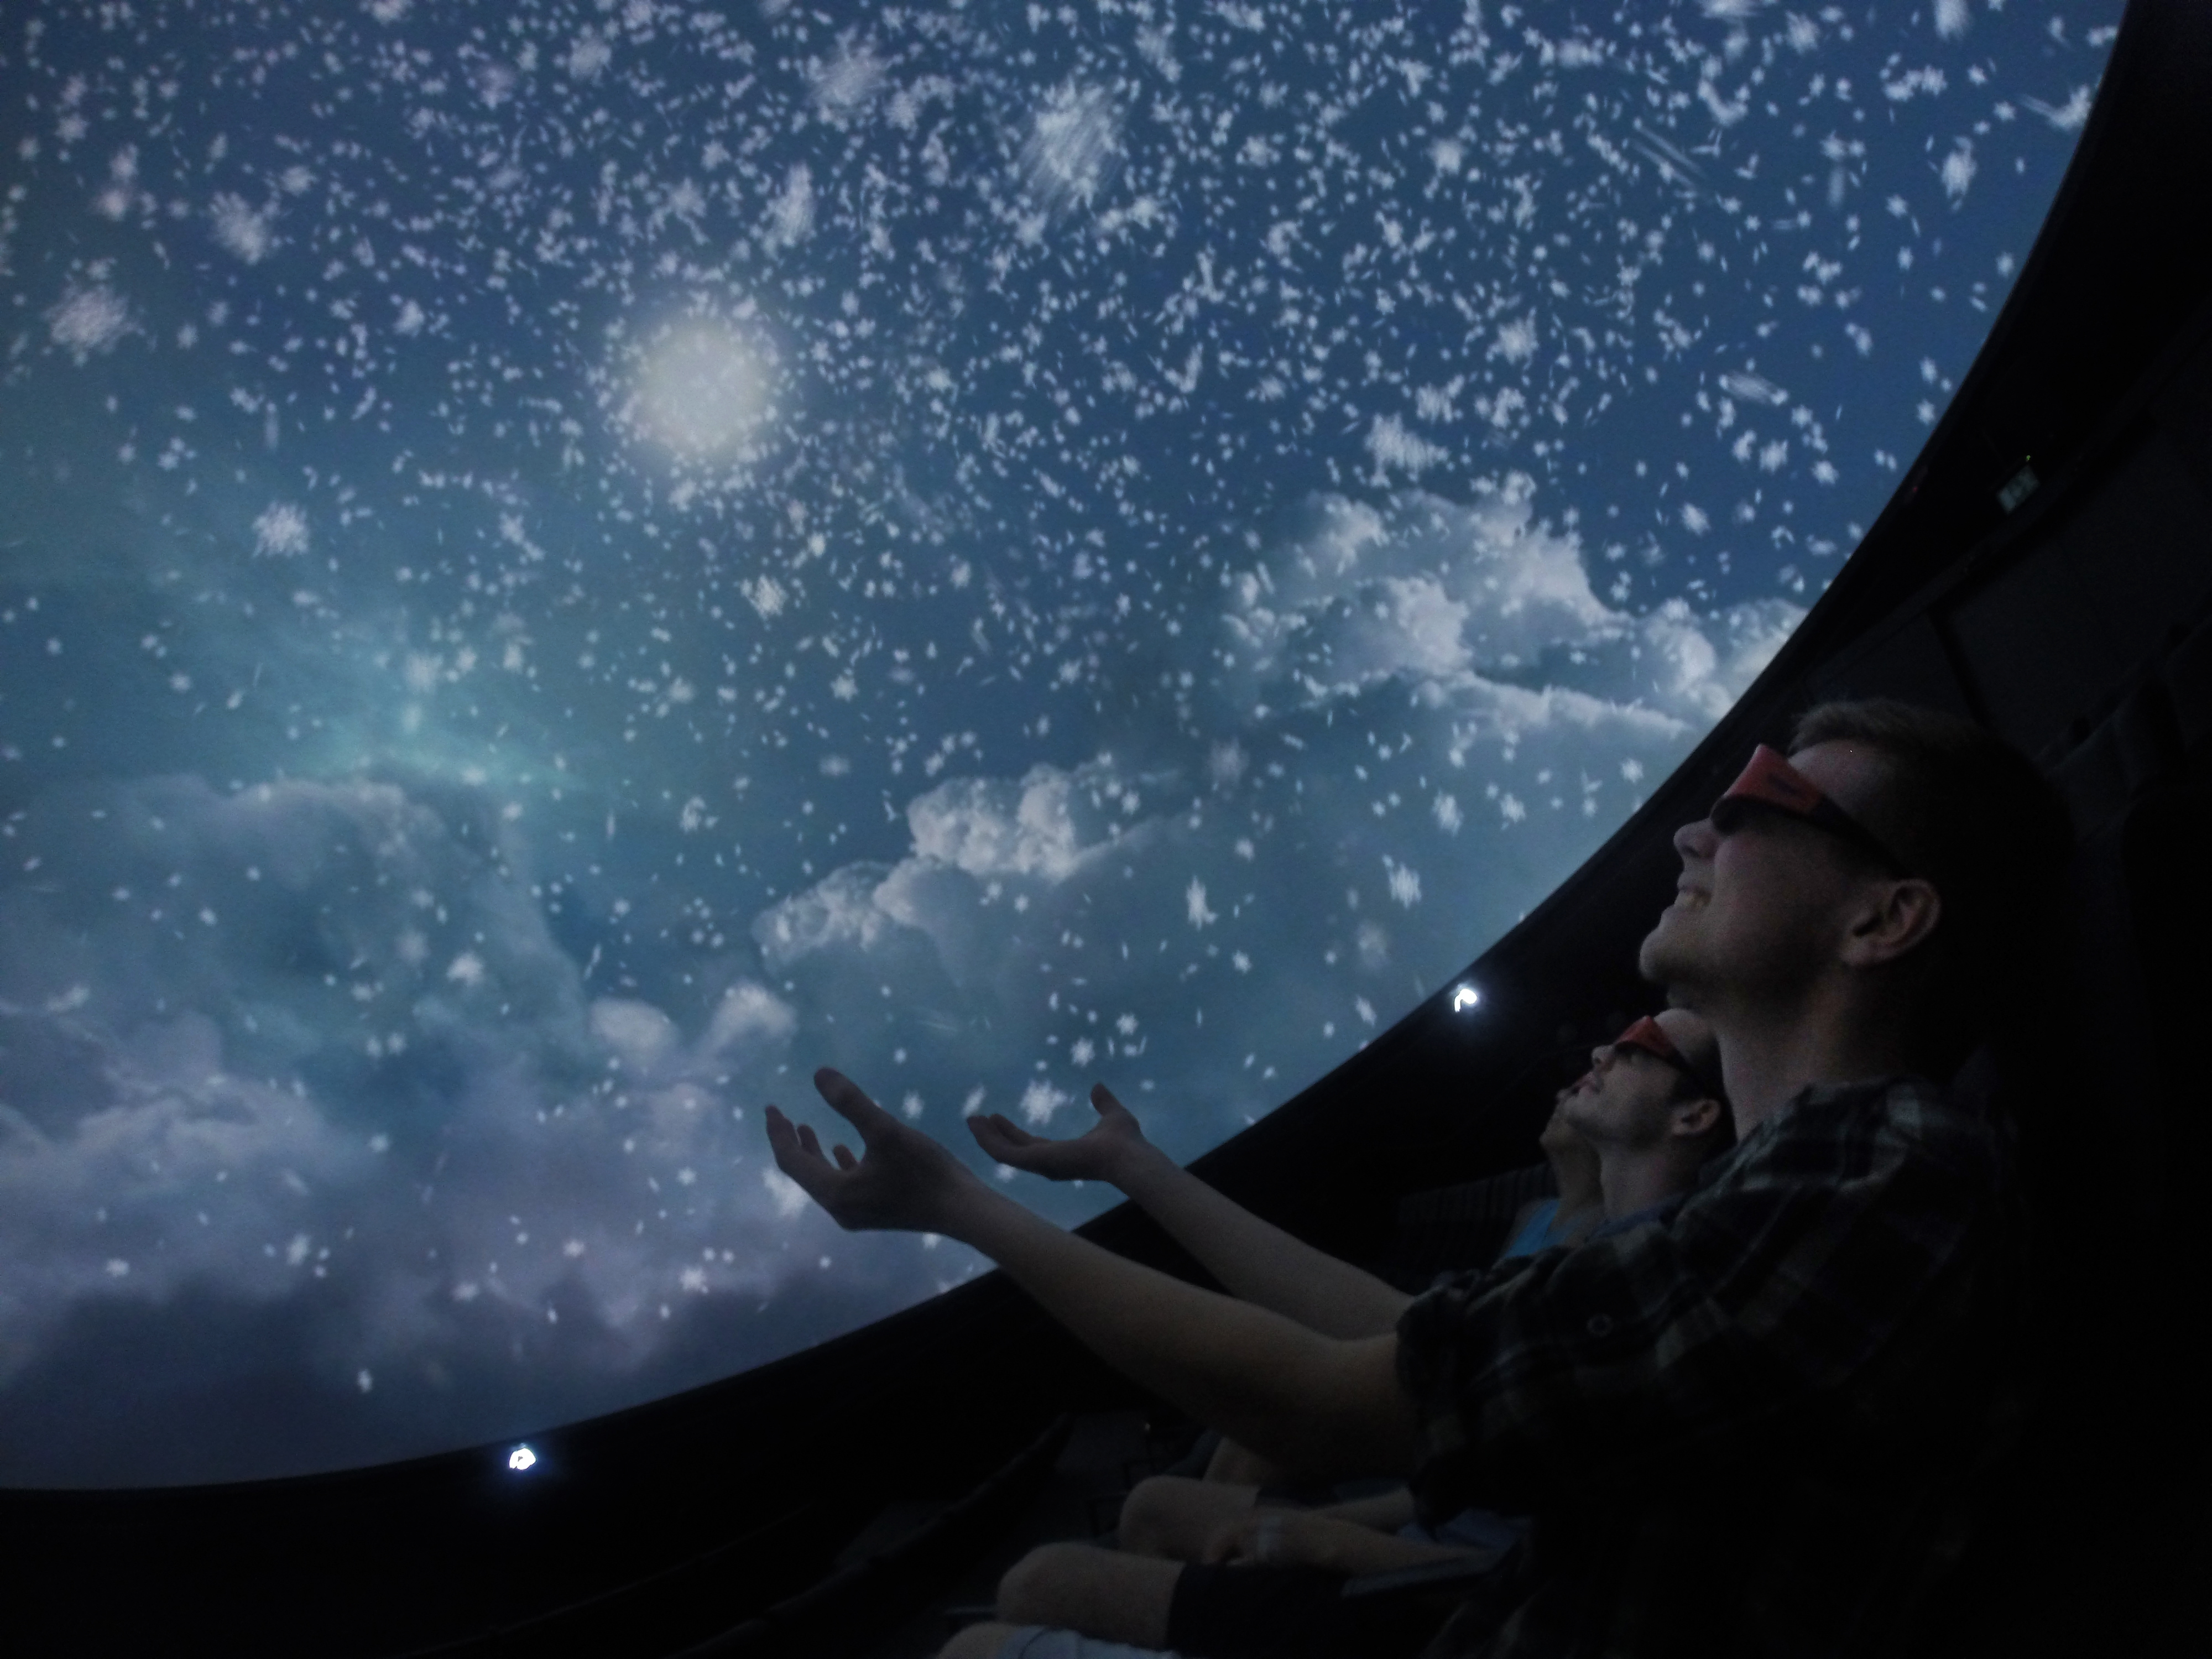
\includegraphics[width=1\textwidth]{modellcarl.jpg}
\end{figure}

\section*{Bakgrund och idé}

	Projektets grundidé handlade om att visualisera olika typer av partikelsystem i domteatern på Visualiseringscenter C. Initialt lades fokus på snösimulering och tanken var att försöka arbeta på ett sådant sätt att vidareutveckling skulle vara möjligt. En tänkt riktning var att skapa olika typer av partikelsystem för att representera de olika årstiderna och visa upp ett år genom att växla simulering.

\section*{Verktyg vi använt och varför vi valde dem}
	För att utveckla programvara för domen användes \emph{SGCT}, \emph{Simple Graphics Cluster Toolkit}. SGCT är ett bibliotek gjort för att skapa och hantera 3D-applikationer för sammankopplade datorer (kluster). Detta bygger på \emph{OpenGL} och är skrivet i \emph{C++}.

	Eftersom utveckling skedde på flera olika plattformar, \emph{Windows 7}, \emph{Windows 8}, \emph{Mac OS X} samt \emph{Linux} fattades beslutet att bygga projektet med hjälp utav \emph{Cmake}. Det är ett program som utifrån en lista med instruktioner kan generera olika projektfiler, som sedan används för att kompilera programmet på alla plattformar. Det kan till exempel handla om \emph{Visual Studio}-projektfiler eller vanliga makefiler för kompilation i terminal. En stor fördel med detta var att buggar och olikheter som kunde uppstå mellan de olika systemen blev lättare att uptäcka.

	För att kontrollera programmet och styra vissa av funktionerna skapades ett enkelt gränssnitt i \emph{C\#}. Gränssnittet skickar parametrar till simuleringen som tar emot datan och applicerar den på noderna i klustret. Alla parametrar synkas för att säkerställa att simuleringen ser likadan ut över hela domen. Med hjälp av detta gränssnitt kunde fältens styrka, partiklarnas storlek och hur nära partiklarna kan komma betraktaren förändras i realtid.

	För att tillsammans jobba med projektet användes versionhanteringsprogrammet \emph{Git} tillsammans med \emph{GitHub}. För att ha koll på vad som skulle göras användes GitHubs \emph{issue}-system.

\section*{Arbetsprocess}
	Arbetet grundades i att ständigt ha något fungerande att tillgå och gruppen strävade efter att utveckla enligt ett agilt tankesätt. Fördelen med detta arbetssätt var att det alltid fanns något att se och det gav en tydlig känsla av att arbetet utvecklades och fördes framåt. Designen av programvaran baserades även på att vara så skalbart som möjligt. Det gjorde att en implementation av ett nytt fält som skulle påverka partiklarna hade liten påverkan på den grundläggande kodbasen.

	För att koppla samman partiklar och fält skapades ett fältsystem. Detta system består utav en lista. För varje ruta går programmet igenom listan och fälten producerar en accelerationsvektor till fälten. Beroende på vad för typ av fält det är påverkas accelerationen av partikelns position.

	För att hantera det antal partiklar som simulerades utnyttjades en metod som kallas instansiering. Det betyder att alla partiklar delar på en gemensam snöflinga och att alla partiklar ritas ut i ett gemensamt \emph{draw call}. Detta gjorde att programmet inte behövde gå från CPU:n till GPU:n för varje partikel vilket var en stor prestandaökning.

	I början av projektets gång skapades ett system för att kunna ladda in modellerade objekt i scenen. Denna funktion behölls men användes ej efter beslutet att det estetiskt inte passade in i scenen. Istället började en funktion för att kunna använda modeller som partiklar utvecklas. Något som inte blev färdigt inom projektets ramar.

\section*{Lärdomar under arbetets gång}
	En lärdom gruppen kunde dra var problematiken med att utveckla på olika plattformar. Bara för att det såg bra ut på en skärm betydde det inte att det fungerade på alla andra. Detta visade sig även vara ett problem när det testades i domen för första gången då gränssnittet bara kunde styra huvudnoden i domen. Eftersom programmet bara hade testats på egna datorer tidigare, var det svårt att förutsäga hur programmet skulle bete sig över flera noder.

	Något som blev uppenbart under detta arbete var att det krävdes väldigt mycket detaljarbete för att skapa en realistisk visualisering. Gränssnittet var till stor hjälp för att göra simuleringen verklighetstrogen och för att upptäcka brister i programmet. Ett beslut gruppen tog under arbetets gång var att bara fokusera på snösimuleringen. Detta för att det inte skulle bli för tungt arbete och för att det i slutändan skulle finnas något bra och komplett att visa upp.

\section*{Resultatet}
	Den färdiga produkten är ett partikelsystem anpassat för att visas i domen, där olika fält kan appliceras för att simulera olika effekter. Vind, virvlar och även gravitation kan skapas och regleras via gränssnittet. Systemet är designat för att göra det enkelt att bygga vidare på och ger användaren möjligheten att själv bestämma hur simulationen ska se ut och bete sig.

\end{document}
